% Version 1.2 of SN LaTeX, November 2022
%
% See section 11 of the User Manual for version history 
%
%%%%%%%%%%%%%%%%%%%%%%%%%%%%%%%%%%%%%%%%%%%%%%%%%%%%%%%%%%%%%%%%%%%%%%
%%                                                                 %%
%% Please do not use \input{...} to include other tex files.       %%
%% Submit your LaTeX manuscript as one .tex document.              %%
%%                                                                 %%
%% All additional figures and files should be attached             %%
%% separately and not embedded in the \TeX\ document itself.       %%
%%                                                                 %%
%%%%%%%%%%%%%%%%%%%%%%%%%%%%%%%%%%%%%%%%%%%%%%%%%%%%%%%%%%%%%%%%%%%%%

%%\documentclass[referee,sn-basic]{sn-jnl}% referee option is meant for double line spacing

%%=======================================================%%
%% to print line numbers in the margin use lineno option %%
%%=======================================================%%

%%\documentclass[lineno,sn-basic]{sn-jnl}% Basic Springer Nature Reference Style/Chemistry Reference Style

%%======================================================%%
%% to compile with pdflatex/xelatex use pdflatex option %%
%%======================================================%%

%%\documentclass[pdflatex,sn-basic]{sn-jnl}% Basic Springer Nature Reference Style/Chemistry Reference Style


%%Note: the following reference styles support Namedate and Numbered referencing. By default the style follows the most common style. To switch between the options you can add or remove “Numbered” in the optional parenthesis. 
%%The option is available for: sn-basic.bst, sn-vancouver.bst, sn-chicago.bst, sn-mathphys.bst. %  
 
%%\documentclass[sn-nature]{sn-jnl}% Style for submissions to Nature Portfolio journals
%%\documentclass[sn-basic]{sn-jnl}% Basic Springer Nature Reference Style/Chemistry Reference Style
\documentclass[sn-mathphys,Numbered]{sn-jnl}% Math and Physical Sciences Reference Style
%%\documentclass[sn-aps]{sn-jnl}% American Physical Society (APS) Reference Style
%%\documentclass[sn-vancouver,Numbered]{sn-jnl}% Vancouver Reference Style
%%\documentclass[sn-apa]{sn-jnl}% APA Reference Style 
%%\documentclass[sn-chicago]{sn-jnl}% Chicago-based Humanities Reference Style
%%\documentclass[default]{sn-jnl}% Default
%%\documentclass[default,iicol]{sn-jnl}% Default with double column layout

%%%% Standard Packages
\usepackage{graphicx}%
\usepackage{multirow}%
\usepackage{amsmath,amssymb,amsfonts}%
\usepackage{amsthm}%
\usepackage{mathrsfs}%
\usepackage[title]{appendix}%
\usepackage{xcolor}%
\usepackage{textcomp}%
\usepackage{manyfoot}%
\usepackage{booktabs}%
\usepackage{algorithm}%
\usepackage{algorithmicx}%
\usepackage{algpseudocode}%
\usepackage{listings}%
\usepackage{pythonhighlight}
%%%%

%%%%%=============================================================================%%%%
%%%%  Remarks: This template is provided to aid authors with the preparation
%%%%  of original research articles intended for submission to journals published 
%%%%  by Springer Nature. The guidance has been prepared in partnership with 
%%%%  production teams to conform to Springer Nature technical requirements. 
%%%%  Editorial and presentation requirements differ among journal portfolios and 
%%%%  research disciplines. You may find sections in this template are irrelevant 
%%%%  to your work and are empowered to omit any such section if allowed by the 
%%%%  journal you intend to submit to. The submission guidelines and policies 
%%%%  of the journal take precedence. A detailed User Manual is available in the 
%%%%  template package for technical guidance.
%%%%%=============================================================================%%%%

%\jyear{2021}%=--

%% as per the requirement new theorem styles can be included as shown below
\theoremstyle{thmstyleone}%
\newtheorem{theorem}{Theorem}%  meant for continuous numbers
%%\newtheorem{theorem}{Theorem}[section]% meant for sectionwise numbers
%% optional argument [theorem] produces theorem numbering sequence instead of independent numbers for Proposition
\newtheorem{proposition}[theorem]{Proposition}% 
%%\newtheorem{proposition}{Proposition}% to get separate numbers for theorem and proposition etc.

\theoremstyle{thmstyletwo}%
\newtheorem{example}{Example}%
\newtheorem{remark}{Remark}%

\theoremstyle{thmstylethree}%
\newtheorem{definition}{Definition}%

\raggedbottom
%%\unnumbered% uncomment this for unnumbered level heads

\begin{document}

\title[Lachi el popular]{Lachi el popular}

%%=============================================================%%
%% Prefix	-> \pfx{Dr}
%% GivenName	-> \fnm{Joergen W.}
%% Particle	-> \spfx{van der} -> surname prefix
%% FamilyName	-> \sur{Ploeg}
%% Suffix	-> \sfx{IV}
%% NatureName	-> \tanm{Poet Laureate} -> Title after name
%% Degrees	-> \dgr{MSc, PhD}
%% \author*[1,2]{\pfx{Dr} \fnm{Joergen W.} \spfx{van der} \sur{Ploeg} \sfx{IV} \tanm{Poet Laureate} 
%%                 \dgr{MSc, PhD}}\email{iauthor@gmail.com}
%%=============================================================%%

\author{\textbf{Lia Zerquera Ferrer},
\textbf{Daniel C\'ardenas Cabrera}}

%%==================================%%
%% sample for unstructured abstract %%
%%==================================%%



%%================================%%
%% Sample for structured abstract %%
%%================================%%

% \abstract{\textbf{Purpose:} The abstract serves both as a general introduction to the topic and as a brief, non-technical summary of the main results and their implications. The abstract must not include subheadings (unless expressly permitted in the journal's Instructions to Authors), equations or citations. As a guide the abstract should not exceed 200 words. Most journals do not set a hard limit however authors are advised to check the author instructions for the journal they are submitting to.
% 
% \textbf{Methods:} The abstract serves both as a general introduction to the topic and as a brief, non-technical summary of the main results and their implications. The abstract must not include subheadings (unless expressly permitted in the journal's Instructions to Authors), equations or citations. As a guide the abstract should not exceed 200 words. Most journals do not set a hard limit however authors are advised to check the author instructions for the journal they are submitting to.
% 
% \textbf{Results:} The abstract serves both as a general introduction to the topic and as a brief, non-technical summary of the main results and their implications. The abstract must not include subheadings (unless expressly permitted in the journal's Instructions to Authors), equations or citations. As a guide the abstract should not exceed 200 words. Most journals do not set a hard limit however authors are advised to check the author instructions for the journal they are submitting to.
% 
% \textbf{Conclusion:} The abstract serves both as a general introduction to the topic and as a brief, non-technical summary of the main results and their implications. The abstract must not include subheadings (unless expressly permitted in the journal's Instructions to Authors), equations or citations. As a guide the abstract should not exceed 200 words. Most journals do not set a hard limit however authors are advised to check the author instructions for the journal they are submitting to.}



%%\pacs[JEL Classification]{D8, H51}

%%\pacs[MSC Classification]{35A01, 65L10, 65L12, 65L20, 65L70}

\maketitle

\section{Descripci\'on del problema}\label{sec1}

\begin{center}
    \textbf{Lachi el popular}
\end{center} 

Lashi ya casi se gradúa y quiere ser popular, para esto es que escogió esta carrera. Planea ser popular creando un grupo solo de gente popular, así el también será popular. En el aula hay varias opiniones de quien no es "cool", por ejemplo Karel puede pensar que Lashi no es "cool", o simplemente no pensar nada, a su vez Lashi puede tener sus opiniones.\\

Como los populares no pueden ser muchos, Lashi tiene que darse a la tarea de crear un grupo de estudiantes populares, no mayores que un entero positivo k, que cumpla que: Nadie piensa que alguien del grupo de los populares no es "cool", a no ser que sea otro popular.

\section*{Inputs}
\textbf{M[n,n]}: una matriz de n x n donde la posición i,j representa la opinión que tiene el estudiante i del estudiante j (si M[i,j] = 0, el estudiante i no opina nada del j, si es uno piensa que es "cool" y si es -1 piensa que "no es cool")\\
\textbf{k} Tama\~no máximo del grupo de los populares
\section*{Oupts}
\textbf{s}: Que es una lista que contiene al grupo de todos los estudiantes populares.

\section*{Nuestro problema es NP ?}

El problema del clique es el problema de optimización que consiste en encontrar una clique de tamaño máximo en un grafo. El problema de decisión correspondiente pregunta simplemente si existe en el grafo un clique de un tamaño determinado.\\
Una solución ingenua para este problema es $\Omega (k^2(\frac{|V|}{k})) $ que es polinomial si k es constante\\
Este problema es NP-Completo, sin embargo con k cercano a $\frac{|V|}{2}$ en este caso el algoritmo corre en tiempo super polinomial.\cite{1}

\subsection {Demostraci\'on de que nuestro problema es equivalente al problema del clique}
Para hacer mas cómoda nuestra modelaci\'on del problema hicimos una peque\~na mo-dificaci\'on en el input en lugar de una matriz de nxn estaremos trabajando con un lista donde en la posición i hay una instancia de la clase Student que contiene a todas personas que i cree que "no son cool". \\
Modelaremos nuestro problema mediante un grafo G que cumple lo siguiente:
\begin{itemize}
    \item $\forall$ u,v $\in V(G) ~\exists <u,v> \in E(G) $ si u opina mal de v la arista $(u,v)$ tendr\'a el atributo "is-negative" \textbf{Fig 1}
\end{itemize}
\begin{figure}[h]
        \centering
        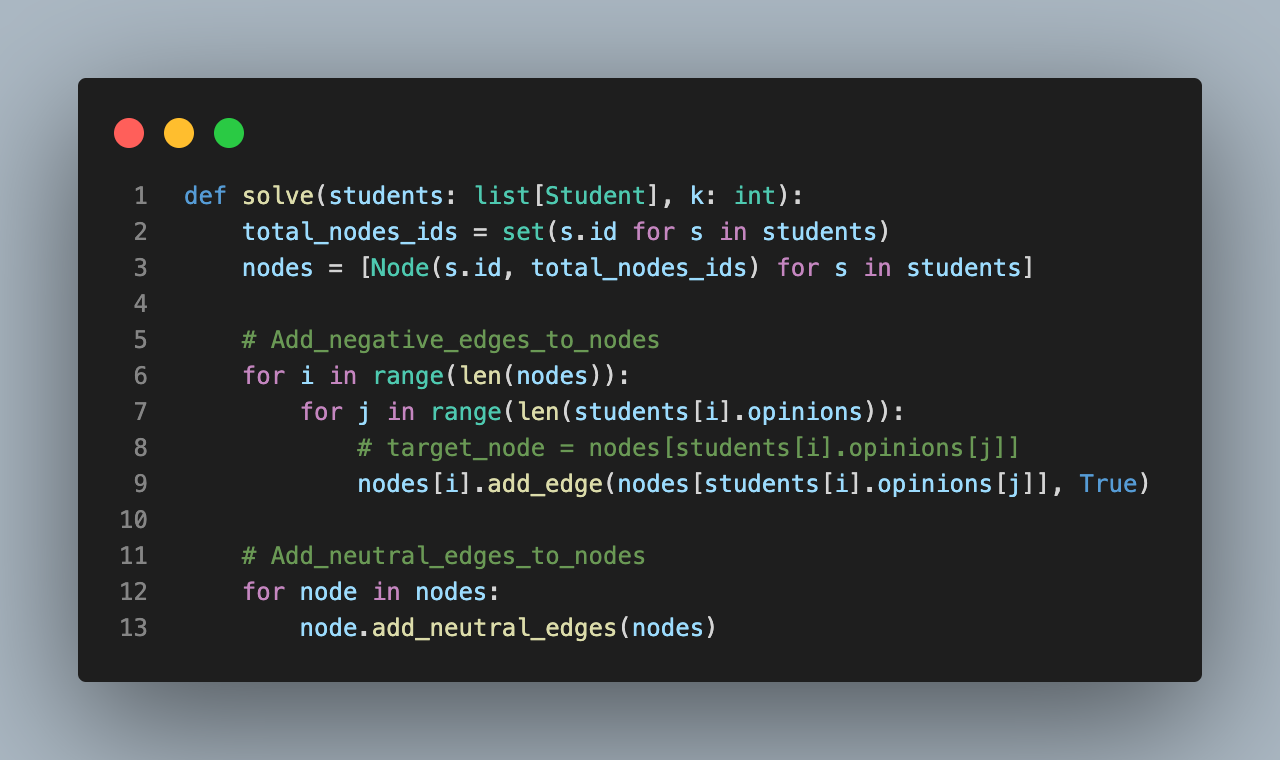
\includegraphics[height=0.3\textheight, width=0.8\textwidth]{build_graph.png}
        \centering
        \caption{Crear el grafo}
\end{figure}
\textbf{Nota 1:} Note que dicho grafo G, es un grafo completo ya que existen aristas entre todo par de vértices de V(G)\\

Entendemos como solución en esta modelaci\'on lo siguiente: una solución factible a nuestro problema es encontrar un clique(C) de tama\~no menor o igual que k tal que para todo $v \in C$ y $u \notin C$ no existe la arista $<u,v>$ con el atributo es "is-negative". En otras palabras nadie que este fuera del clique piensa que alguien dentro del clique "no es cool".\\

Note que una manera ingenua de obtener una solución de nuestro problema es obtener todos los cliques de tama\~no k del grafo, esto podemos hacerlo de la siguiente manera aplicamos el algoritmo que da solución al problema del clique sobre G obteniendo $k_1$ y luego volvemos a aplicar dicho algoritmo en el grafo $G_1 = G - K_1$ resultante y así sucesivamente hasta que no sea posible encontrar un clique de tama\~no k.\\ 
\textbf{Nota 2:} Note que encontrar todos los cliques de tama\~no k es resolver el problema del clique un nu\'mero finito de veces por tanto este problema es NP.\\
Una vez que tenemos que tenemos todos los cliques de tama\~no k nos quedamos con el primero que cumpla la condición de factibilidad. Si ninguno de tama\~no k lo cumple, pues repetimos el mismo procedimiento para k - 1. Si llegamos a k = 0 devolvemos una lista vacía.\\
Note que nuestra solución ingenua es $\Omega (k^3(\frac{|V|}{k})) $ ya que a lo sumo aplicamos el algoritmo del clique k veces.
\subsection*{Detalles de implementación y code}
A la hora de la implementación notamos la siguiente invariante y es que podemos ir construyendo el clique verificando que cada nodo que a\~nadimos cumple que adem\'as de estar conectados con todos cumple la condición de factibilidad.\\
Esto har\'ia a nuestro algoritmo ganar en eficiencia.\\
A continuaci\'on explicamos el algoritmo: \\ 
Tomamos un nodo i cualquiera del grafo y lo a\~nadimos al nuestro grupo de populares junto con todos los que piensan que i "no es cool" ,llamémosle a este conjunto de nodos A, luego iteramos por el conjunto A y por cada nodo realizamos el mismo procedimiento, entrar en en el clique y a\~nadir a A todos los nodos que piensan que $A_i$ "No es cool" y así sucesivamente hasta que todos cumplan la condici\'on de factibilidad. Luego si $|A| < k$ probar añadir un estudiante del conjunto $V - A$ y repetir el proceso\\

En caso de que no se cumpla la condición de factibilidad llevamos una variable global que guarda el mejor clique(el de mayor tama\~no encontrado hasta el momento que sea a su vez menor o igual que k) comparamos el mejor clique encontrado empezando por i y si es necesario se actualiza la variable global.\\
Luego se repite el proceso con un nodo $j \neq i$.\\
 En caso de nunca encontrar un clique de tama\~no menor o igual que k que cumpla la condici\'on de factibilidad, devolvemos una lista vac\'ia.\\
\begin{figure}[h]
        \centering
        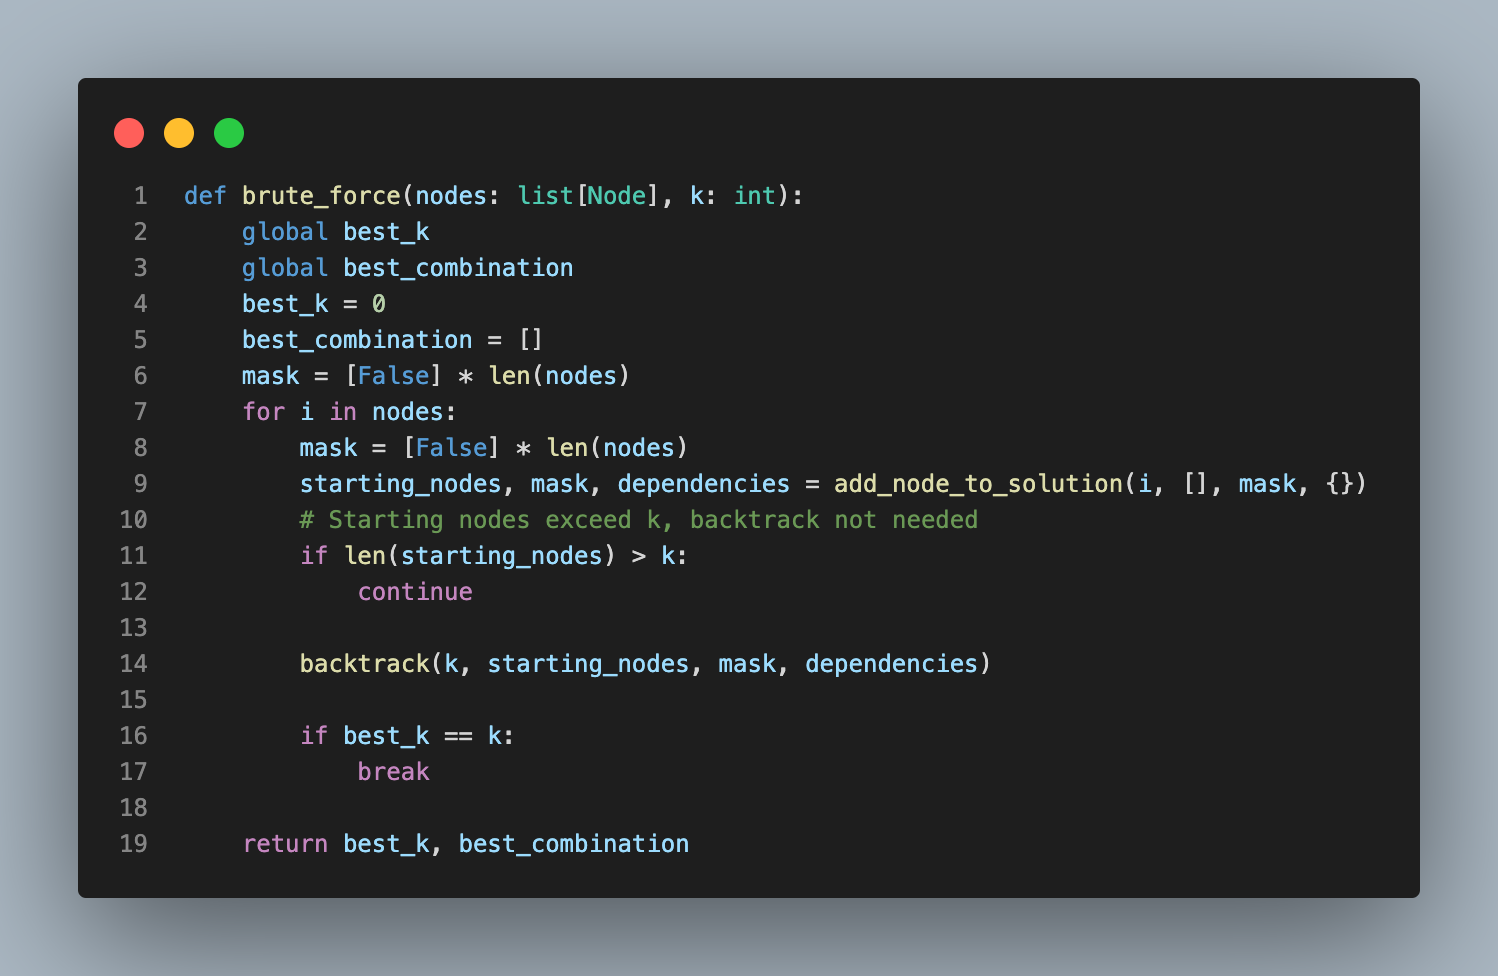
\includegraphics[height=0.3\textheight, width=0.8\textwidth]{brute_force.png}
        \centering
        \caption{Algoritmo de fuerza bruta}
\end{figure}

\section{Experimentación con un algoritmo de aproximación }
Nuestra propuesta es utilizar la metahur\'istica Colonia de Hormigas para resolver el problema de encontrar el clique de tama\~no máximo menor o igual que k.\\
Implementamos un algoritmo de aproximación de forma tal que genera cliques máximos\footnote{Se conoce como clique m\'aximo aquel que no esta contenido en ning\'un otro clique} mediante la adición repetida de vértices a cliques parciales\footnote{Se conoce como clique parcial aquel que esta contenido totalmente en alg\'un clique distinto de si mismo}.\\
La metahur\'istica colonia de hormigas(ACO) es un enfoque bio-inspirado que se ha utilizado para resolver problemas de optimizaci\'on combinatoria dif\'iciles\cite{2,3}.La idea principal de ACO es buscar un camino de costo mínimo en grafo G. Hormigas artificiales caminan a través de dicho grafo buscando "buenos caminos". Se encuentran mejores caminos debido a la cooperaci\'on entre hormigas de la colonia. Esta cooperación se realiza de forma indirecta a través de la colocaci\'on de feromonas.\\
El algoritmo ACO propuesto para encontrar cliques máximos lo denominamos AntClique y lo explicamos a continuaci\'on:\\
\begin{itemize}
    \item Primero debemos analizar la inicializaci\'on de feromonas, las hormigas se comunican a través de la feromonas en las aristas del grafo. La cantidad de feromonas en el la arista (u,v) es denotada por \textit{t}(u,v) y representa el peso aprendido de que u y v estén en el mismo ciclo.\\
    Como es propuesto en \cite{4,5} imponemos explícitamente limites inferiores y superiores de \textit{t}($\textit{t}_{min}, \textit{t}_{max}$) en los rastos de feromonas, de esta manera se logra una mayor exploraci\'on del espacio de b\'usqueda evitando que las diferencias relativas entre la cantidad de feromonas sean demasiado grandes durante el procesamiento.\\
    Decidimos inicializar las feromonas con el $\textit{t}_{max}$, esta inicialización permite una mayor exploración del espacio de búsqueda durante los primeros ciclos, ya que todas las aristas tienen casi la misma cantidad de feromona durante los primeros ciclos\cite{6}.
    \item Como construir cliques con las hormigas, las hormigas seleccionan un nodo inicial random y a continuaci\'on eligen de forma iterativa los nodos que se van a\~nadiendo al clique (C), dentro de un conjunto de candidatos, que contiene todos los vértices conectados a cada vértice del clique.\\
    La elecci\'on del vertice $v_i$ dentro del conjunto de candidatos, depende de un factor de feromonas $\textit{T}_C(v_i)$. Una diferencia notable con muchos algoritmos ACO es que este factor no sólo depende del rastro de feromonas entre el último vértice añadido en C y el vértice candidato $v_i$, sino de todos los rastreos de feromonas entre C y $v_i$\footnote{El factor de feromonas $\textit{T}_C(v_i)$ es computado de manera incremental, al principio cuando C solo contiene el nodo inicial $\textit{T}_C(v_initial)$  es inicializado con $\textit{t}(v_initial,v_i)$ entonces cada vez que se a\~nade un vértice $v_k$ al clique $\textit{T}_C(v_i)$ se incrementa con $\textit{t}(v_k,v_i)$ } $\textit{T}_C = \sum_{v_j \in C} = \textit{t}(v_i,vj)$ \cite{5}.
    \item Actualizar rastro de feromonas, luego de que cada hormiga construye un clique, el rastro de feromonas es actualizadas, primero a cada rastro de feromonas se le resta un valor simulando la evaporación de feromonas, por cada arista $(u,v) \in E $ la cantidad de feromonas que contiene $\textit{t}(u,v)$ se multiplica por un par\'ametro de evaporaci\'on $\lambda$ tal que $0 \leq \lambda \leq 1$, entonces la mejor hormiga del ciclo deposita feromonas, sea $C_k$ el mayor clique construido durante el ciclo menor o igual que k, y $C_{best}$ la mayor clique menor o igual que k construido desde el principio del recorrido, para cada pareja de vértices $(u,v) \in C_k$, incrementamos la cantidad de feromonas en $\textit{t}(u,v)$ por $\frac{1}{1 + |C_{best}| - |C_k|}$.\cite{5}\\
\end{itemize}
\subsection*{Resultados de la experimentaci\'on}
Hicimos un test-generator para poder probar nuestro algoritmo de aproximaci\'on con varios ejemplos, debido a que nuestro algoritmo naive no es eficiente no se pudieron generar casos de pruebas muy grandes, por tanto la poblaci\'on de estudiantes varia entre los 5 y 50 estudiantes.\\
Con poblaci\'on peque\~nas resulta que nuestro algoritmo de aproximaci\'on  coincide en su totalidad con el resultado obtenido con la fuerza bruta \textbf{Fig 3}.\\

\begin{figure}[h]
        \centering
        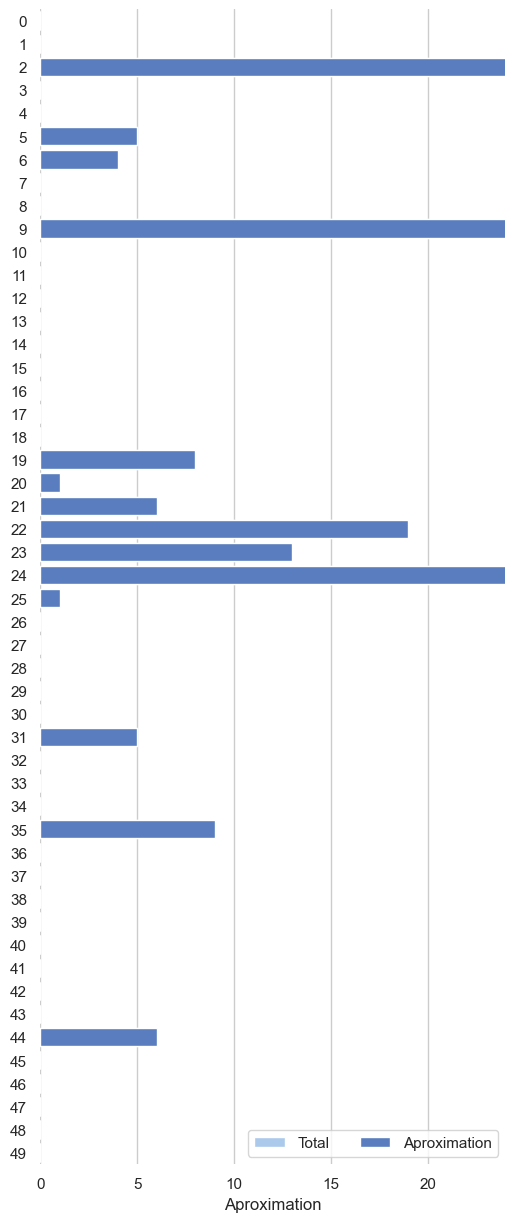
\includegraphics[height=0.5\textheight, width=0.8\textwidth]{Untitled.png}
        \centering
        \caption{Resultados de la experimentaci\'on}
\end{figure}
\begin{thebibliography}{99}
\bibitem{1} thomas-h-cormen-introduction-to-algorithms-4th-edition parte VII cap #4.5 page 1082 Theorem 34.11
 \bibitem{2} M. Dorigo. Optimization, Learning and Natural Algorithms (in Italian). PhD thesis, Dipartimento di Elettronica, Politecnico di Milano, Italy, 1992
 \bibitem{3} M. Dorigo, G. Di Caro, and L. M. Gambardella. Ant algorithms for discrete opti- mization. Artificial Life, 5(2):137–172, 1999.
\bibitem{4}T.StutzleandH.H.Hoos.MAX−MINAntSystem.JournalofFutureGeneration Computer Systems, 16:889–914, 2000.
\bibitem{5} Searching for Maximum Cliques with Ant Colony Optimization Serge Fenet and Christine Solnon
\bibitem{6}T.StutzleandH.H.Hoos.MAX−MINAntSystem.JournalofFutureGeneration Computer Systems, 16:889–914, 2000


\end{document}



